\part{Cours Magistral 2 -- Les intégrales}
\section{Utiliser/Généraliser Fubini}
Voir Figure 14.13(a)

Le domaine d'intégration représente un cercle sur le plan x-y. On définit $a$ et $b$, les deux limites du domaine sur l'axe des x (voir (a) ci-dessous).

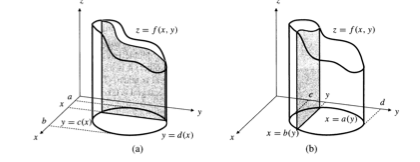
\includegraphics[scale=0.8]{image1.png}

Nous allons calculer l'intégrale d'abord selon y-simple (Figure (a)) puis selon x-simple (Figure (b)) puis comparer les résultats obtenus.
\paragraph{Y-simple}
On note $A(x)$ la surface de l'aire grisée de l'image $(a)$.
\[A(x)=\int_{c(x)}^{d(x)}f(x,y)\dif y\]
$\int_a^b A(x) \dif x$ est un petit élément de volume.

\[\int_a^b A(x) \dif x = \text{Volume de }S = \int_Df(x,y) \dif x \dif y\]

On pourra calculer le volume comme ceci :

\[ \iint_D f(x,y) \dif x \dif y = \int_a^b \int_{c(x)}^{d(x)} f(x,y)  \dif y \dif x = \int_a^b \dif x \int_{c(x)}^{d(x)} f(x,y) \dif y \]

On calcule d'abord l'intérieur (\textit{``Inner''} en anglais) de l'intégrale pour ensuite trouver l'extérieur ((\textit{``Outer''}).
\begin{myrem}
``\emph{x}'' est considéré comme une constante dans l'intégrale ``intérieure''.
\end{myrem}

\paragraph{X-simple}

Voir Figure 14.13(b)
\[\iint_D f(x,y) \dif x \dif y = \int_c^d\int_{a(y)}^{b(y)} \dif x f(x,y)\]
Nous avons le même résultat.\\
En pratique, on a souvent un domaine x-simple et y-simple ! Les deux calculs donneront le même résultats. Mais il y a presque toujours un sens de coupe qui est plus facile que l'autre. Voir exemple ci-dessous.

\subsection{Exemple 1}
\[ I=\iint_D xy \dif x \dif y \]
\begin{center}

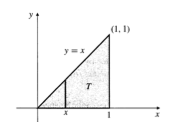
\includegraphics[scale=1]{image2.png}

\end{center}
Commençons par calculer selon \textbf{y-simple}
Les deux bords sont $y=0$ et $y=x$. Le domaine est y-simple. On se fixe un x et on fait la coupe verticalement (dans ce cas). Le point d'entrée est $y=0$ et le point de sortie est $y=x$.
\[I=\int_0^1 dx \int_0^x \dif y(xy)\]
Or on peut calculer l'intégrale interne
\[\int_0^x dy(xy) = \left[ x \frac{y^2}{2} \right]_0^x = \frac{x^3}{2}\]
On aura donc au final
\[I=\int_0^1\frac{x^3}{2} \dif x = \left[\frac{x^4}{8}\right]_0^1= \frac{1}{8}\]

On peut aussi calculer selon \textbf{x-simple}.
\\
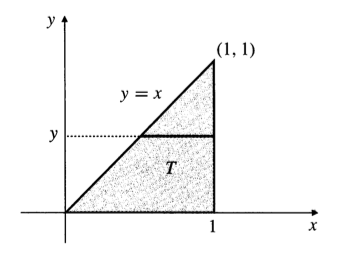
\includegraphics[scale=0.5]{image3}
\\

Le point d'entrée est $x=y$ et le point de sortie est $x=1$.
\[I=\int_0^1\dif y\int_y^1\dif x(xy)\]

Au sein de l'intégrale interne, y est constant.

\[\int_y^1\dif x(xy) = \frac{y}{2}(1-y^2)\]
Au final, on trouve l'intégrale.
\[I = \int_0^1 \frac{y}{2}(1-y^2) \dif y = 1/8\]

On a le même résultat si l'on considère le domaine x-simple ou y-simple!

\subsection{Exemple 2}
\[I = \int_0^1\dif x \int_{\sqrt{x}}^1 \dif y e^{y^3}\]

On voit que la variable x est entre 0 et 1 et que la variable y ne va pas plus haut que 1.
\\
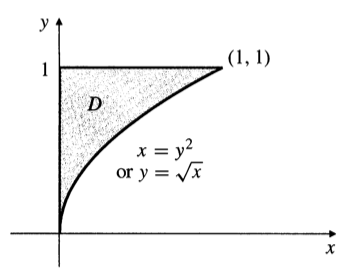
\includegraphics[scale=0.5]{image4.png}
\\

En regardant le domaine, on se rend compte qu'il est x-simple et y-simple !
\begin{itemize}

\item Les bords en x sont $x=0$ et $x=y^2$
\item Les bords en y sont $y=1$ et $y=\sqrt{x}$


\end{itemize}

\[I \overset{aussi}{=}\int_0^1dy \int_0^{y^2} dx e^{y^3}\]
\[\int_0^{y^2} dx e^{y^3} = e^{y^3} \int_0^{y^2} dx = e^{y^3} x \Big|_0^{y^2} = y^2 e^{y^3}\]
\[I=\int_0^1 y^2 e^{y^3} dy = \left[1/3 e ^{y^3}\right]_0^1  = \frac{e-1}{3}\]
Parce que
$y^2 e^{y^3} = \frac{d}{dy}(\frac{1}{3} e^{y^3})$

\section{Changement de variables}
Nous allons commencer par montrer un exemple pour prouver l'utilité du changement de variable pour ensuite passer au cas général.
\subsection{Exemple}
\[I=\int_D (1-x^2-y^2)\]
\begin{center}
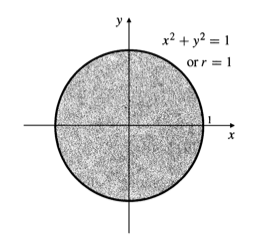
\includegraphics[scale=0.7]{image5.png}
\end{center}

 En y, le point d'entrée est $y=-\sqrt{1-x^2}$ et la sortie est  $y=\sqrt{1-x^2}$ ( pendant que x varie entre -1 et 1)

 \[I=\int_{-1}^1 \dif x \int_{-\sqrt{1-x^2}}^{\sqrt{1-x^2}} \dif y(1-x^2-y^2) \]

 \begin{myrem}
 $$\left\{
 \begin{array}{r}
 x=r\cos\Theta = \tilde{x}(r,\Theta)\\
 y=r \sin \Theta = \tilde{y}(r,\Theta)
 \end{array}
 \right.
 $$

 Exprimer f(x,y) en fonction de $(r,\Theta)$
 
 Calculer l'élément infinitésimale d'aire $\dif A$
 \end{myrem}

 On change donc de variables
 \[f(x,y)=1-x^2-y^2=f(x(r,\Theta),y(r,\Theta)) = g(r,\Theta)\]
 \[f(x,y) = 1-r^2\cos^2\Theta -r^2\sin^2\Theta = 1-r^2 = g(r,\Theta)\]
 \begin{center}

 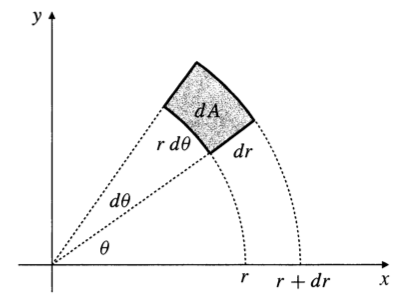
\includegraphics[scale=0.7]{image6.png}\\

 \end{center}
 Que vaut le petit élément $dA$ ? On considère que c'est un parallèlogramme.
 $\dif A\approx (rd\Theta)\times \dif r$
 \[\dif A = r \dif r \dif\Theta\]

 A présent, tout devient plus simple ! L'intégrale qui nous interesse devient donc
 \[I=\int_S (1-r^2)r \dif r \dif\Theta\]
\begin{center}
 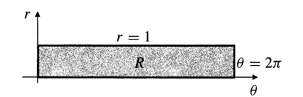
\includegraphics[scale=0.7]{image7.png}
\end{center}
 \[I=\int_0^{2\pi} \dif\Theta \int_0^1 \dif r r (1-r^2)\]
 \[I = \int_0^{2\pi} \dif \Theta \left(\frac{r^2}{2}-\frac{r^4}{4} \right) \text{évalué entre 1 et 0} = \frac{1}{4} \int_0^{2\pi} \dif \Theta = \pi/2 \]

\subsection{Cas général}

$$x=x(u,v)$$
$$y=y(u,v)$$
\begin{center}
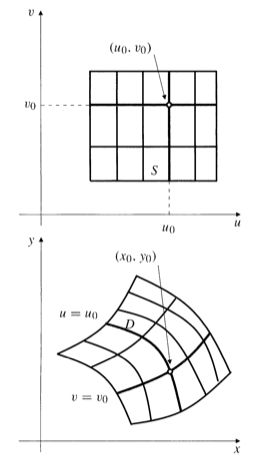
\includegraphics[scale=0.5]{image8.png}
\end{center}

On trace une courbe sur le deuxième graphique qui représente l'ensemble des points où $u=u_0$ est constant. Même chose pour $v=v_0$\\
Ce qui explique ce pavage \og courbé\fg{}. On appelle ça du \textit{``mapping''}. Mais dans le cas d'un changement de variable, on veut que cette transformation soit bijective.\\

On peut donc trouver
$u=u(x,y)$
$v=v(x,y)$
\subsection{Jacobienne de la transformation}

Pour effectuer un changement de variable, il faut calculer la jacobienne du changement de variable défini comme suit (voir la suite pour savoir comment l'utiliser)

\[\tilde{J}=\frac{\partial ( u,v)}{\partial ( x,y) }\]

\[\tilde{J} =
\begin{vmatrix}
\frac{\partial u}{\partial x} &\frac{\partial u}{\partial y}\\
\frac{\partial v}{\partial x} &\frac{\partial v}{\partial y}\\
\end{vmatrix}
\]

On cherche donc la matrice $$J=\dfrac{1}{\tilde{J}}=\frac{\partial ( x,y) }{\partial ( u,v)}$$


$$J = \begin{vmatrix}
\frac{\partial x}{\partial u} &\frac{\partial y}{\partial u}\\
\frac{\partial x} {\partial v}&\frac{\partial y}{\partial v}
\end{vmatrix}$$


\[\iint_D f (x,y) \frac{\dif A}{\dif x\dif y}=\iint_S g(u,v) \dif A\]

\begin{center}
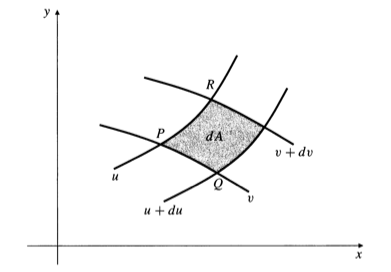
\includegraphics[scale=0.7]{image9.png}
\end{center}

\paragraph{P}
$$x(u,v)$$
$$y(u,v)$$
\paragraph{Q}
\[x(u+\dif u,v)=x(u,v)+\frac{\partial x}{\partial u} \dif u\]
\[y(u+\dif u,v)=y(u,v)+\frac{\partial y}{\partial u} \dif u\]
\paragraph{$\vec{PQ}$}

$$ \vec{PQ} = \left( \frac{\partial x}{\partial u} \dif u\right) \xunit +\left( \frac{\partial y}{\partial u} \dif u \right) \yunit $$
\paragraph{$\vec{PR}$}
$$\vec{PR} = \left(\frac{\partial x}{\partial v} \dif v \right) \xunit + \left( \frac{\partial y}{\partial v} \dif v \right) \yunit $$

Toutes les $ \frac{\partial .}{\partial .} $ sont calculées en $(u,v)$
\[\dif A \approx \norm{\vec{PQ} \times \vec{PR}}\]

\[ \norm{
\begin{vmatrix}
\xunit & \yunit & \zunit\\
\left(\frac{\partial x}{\partial u} \dif u \right) & \left(\frac{\partial y}{\partial u} \dif u \right) & 0 \\
\left(\frac{\partial x}{\partial v} \dif v \right) & \left(\frac{\partial y}{\partial v} \dif v \right) & 0

\end{vmatrix}}
\]

\[=\norm{\frac{\partial x}{\partial u} \frac{\partial y}{\partial v} - \frac{\partial x}{\partial v} \frac{\partial y}{\partial u} \dif u \dif v \zunit}\]
\[= \dif A = \abs{J}\dif u\dif v\]

\fbox{
\begin{minipage}{10cm}

\textbf{Formule à connaître \# 1}

Cette formule est primordiale lors du calcul d'une intégrale avec un changement de variables.

\[\iint_D f(x,y)\dif x\dif y = \iint_S g(u,v) \abs{\frac{\partial (x,y)}{\partial (u,v)}} \dif u\dif v\]

\[x=x(u,v) \text{ et }  y = (u,v)\]

\[ D \longleftrightarrow S \]
Il doit y avoir une bijection entre les variables de départ et les variables de fin.\\
\textit{La valeur absolue nous offre la liberté de choisir l'ordre des lignes et des colonnes de la jacobienne.}
\end{minipage}
}

\subparagraph{Exemple}



$$x=x(u,v)=x(r,\Theta)=r\cos(\Theta)$$
$$y=y(u,v)=y(r,\Theta)=r\cos(\Theta)$$





\[
\frac{\partial (x,y)}{\partial (r, \Theta)} =
\begin{vmatrix}
\frac{\partial x}{\partial r}& \frac{\partial x}{\partial \Theta}\\
\frac{\partial y}{\partial r}& \frac{\partial y}{\partial \Theta}
\end{vmatrix}
\]

$$\begin{vmatrix}
\cos\Theta & -r\sin\Theta\\
\sin\Theta & R\cos\Theta
\end{vmatrix}$$
\[=r\cos^2\Theta +r\sin^2\Theta = r > 0\]
$$\dif A = \abs{J}\dif u\dif v \overset{ici}{=}r \dif r \dif\Theta $$

\begin{myrem}

Voir~\cite{adams2013calculus} page~816 ex.~11 % FIXME ce n'est pas la bonne page
\end{myrem}

\subsection{Changement de variables $ \iiint_D $}
$$
\left\{
\begin{array}{l}
x=x(u,v,w)\\
y=y(u,v,w)\\
z=z(u,v,w)\\
\end{array}
\right.
$$

$D \longleftrightarrow S $

\[\int_D f = \int_S f (x(u,v,w),y(u,v,w),z(u,v,w) \dif V\]
\[f (x(u,v,w),y(u,v,w),z(u,v,w)) = g(u,v,w)\]

\[\dif V=\abs{\frac{\partial(x,y,z)}{\partial(u,v,w)}}\dif u\dif v\dif w\]



\subsubsection{Coordonnées sphériques}

Le passage aux coordonnées sphériques est un changement de variable $\iiint_D$
\begin{myrem}

Voir les images 14.45,14.47,14.50,14.52
\begin{figure}


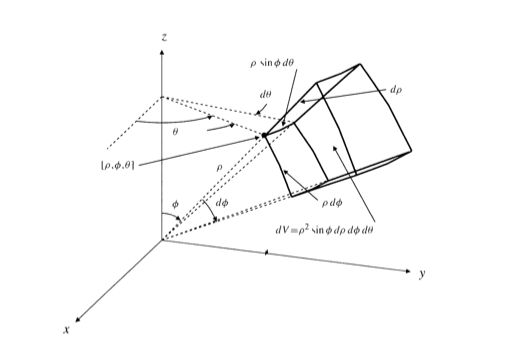
\includegraphics[scale=0.5]{image10.png}
\caption{14.45}
\end{figure}

\begin{figure}
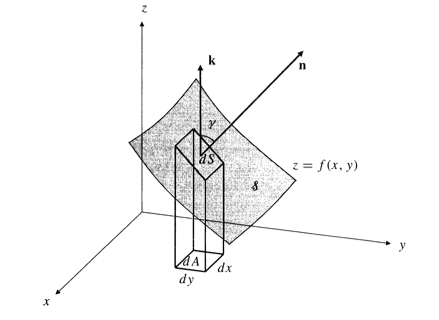
\includegraphics[scale=0.5]{image11.png}
\caption{14.47}
\end{figure}

\begin{figure}
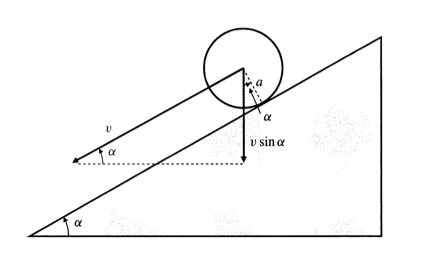
\includegraphics[scale=0.5]{image12.png}
\caption{14.50}
\end{figure}


\end{myrem}
$$
\left\{
\begin{array}{l}

x=g\sin\phi \cos\Theta\\
y=g\sin\phi \sin\Theta\\
z=g\cos\Theta

\end{array}
\right.
$$

est un exemple de changement de variable sphérique.
\[\dif V=g^2\sin\phi \dif g\dif\phi \dif\Theta \]

Faire l'exercice F14.42(b) !



\section{Moyenne d'une fonction}
$f\text{D} \subset \Re ^n$ et on a aussi $\overline{f} = $ moyenne de $f$ constante sur $D$

\[\int_D \overline{f} \eqdef \int_D f = \overline{f}\int_D 1 = \overline{f}\text{Vol(D)}\]

$$\Rightarrow\ \overline{f} = \frac{\int f}{\text{Vol(D)}}$$
\begin{itemize}
\item \textbf{1D} $\overline{f}=\frac{1}{L}\int f$
\item \textbf{2D} $\overline{f}=A^{-1}\iint f$
\item \textbf{3D} $\overline{f} = V^{-1}\iiint f$
\end{itemize}
